\thispagestyle{fancy}
	
	\vspace{-2em} % Adjust vertical space as needed
	\begin{center}



\addcontentsline{toc}{subsection}{Message of the Dean, Faculty of Industrial Technology}    
\subsection*{\textsc{Message of the Dean, Faculty of Industrial Technology}}
	\end{center}

   
    
    \begin{wrapfigure}{l}{0.3\textwidth}
		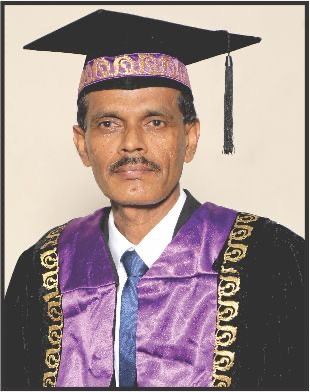
\includegraphics[width=0.3\textwidth]{Images/DeanFIT.jpeg}
	\end{wrapfigure}
	\vspace{2em} % Adjust vertical space as needed




	
	Greetings from the 2024 International Research Symposium, an exciting platform for innovation, learning, and collaboration. On behalf of the Faculty of Industrial Technology, it is my great honor to address all of you as we gather to explore groundbreaking research and insights across diverse fields.
Our faculty consists of four dynamic departments: Film and Television Production Technology, Agriculture and Food Technology, Industrial Management, and Quantity Surveying. These departments drive our mission of nurturing future leaders equipped with the knowledge, skills, and entrepreneurial spirit to meet the evolving needs of industries worldwide.

We provide six Bachelor of Technology degree programs that are uniquely tailored to meet industry standards: Media and Arts Production Technology, Film and Television Production Technology, Food Process Technology, Industrial Management, Hotel Management, and Quantity Surveying. In order to ensure that our graduates not only succeed in their chosen disciplines but also possess the abilities to innovate, adapt, and lead in the rapidly evolving technological landscape, our academic programs place a strong emphasis on techno-entrepreneurship. At the Faculty of Industrial Technology, we are committed to fostering a research and innovation culture among our students and faculty members. This symposium reflects our ongoing efforts to promote academic excellence, encourage knowledge sharing, and inspire new solutions to the challenges facing industries today.

I urge everyone to think creatively and courageously as we have meaningful conversations and share ideas. Let's work together to influence industry, science, and technology in order to create a sustainable and prosperous future.

	
	\vspace{1cm}
	Dr. Kamal Edirisinghe\\
Dean\\
Faculty of Industrial Technology